\documentclass{tufte-handout}
\usepackage{amsmath,amsthm}

\input{vc.tex}

\usepackage{pgfplots}
\pgfplotsset{width=\textwidth,compat=1.5.1}

\newtheorem{claim}{Claim}[section]
\title{\sf Pagerank}
%\date{\GITAuthorDate}
%\author{Thore Husfeldt}

\begin{document}
\maketitle
\footnotetext{rev. \GITAbrHash}

\section{Pagerank}

\begin{marginfigure}
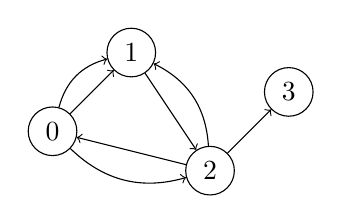
\begin{tikzpicture}
\node (0) [draw,circle] at (0,0) {0};
\node (1) [draw,circle] at (1,1) {1};
\node (2) [draw,circle] at (2,-.5) {2};
\node (3) [draw,circle] at (3,.5) {3};
\draw [->] (0) to [bend left] (1);
\draw [->] (0) to  (1);
\draw [->] (0) to [bend right] (2);
\draw [->] (1) to  (2);
\draw [->] (2) to  (0);
\draw [->] (2) to [bend right] (1);
\draw [->] (2) to (3);
\end{tikzpicture}
\caption{A directed multigraph.}
\end{marginfigure}
Consider an finite, directed multigraph $G=(V,E)$ without self-loops, as in
Fig.~1.
We will understand $G$ as the hyperlink structure of the web pages
described by $V$; an an arc from vertex $u$ to vertex $v$ describes a
hyperlink from page $u$ to page $v$.

The \emph{random surfer} model is a stochastic process that aims to
rank the relevance of a these pages.
The states of this process are the vertices $V$.
With good probability $\alpha$, the process picks an outgoing edge at
random and moves to that page.
(Note that outgoing edges are counted with multiplicities, so from
vertex~1 in the example, the chance of going to 3 is double that of
going to 4.)
Alternatively, with probability $(1-\alpha)$, the surfer becomes bored
and moves to a random page from $V$ instead.
The probability $\alpha$ is called the \emph{damping factor}; a
typically value that works well for web pages is $\alpha = \frac{85}{100}$. 

This process is a finite, irreducible, and ergodic Markov chain.
Its stationary distribution describes the \emph{page rank} of each
vertex. The contribution of Serge Brin and Larry Page was to
realise that this value gives a good measure of the relevance of a web
page, which is the main idea behind the search engine Google.

\subsection{Files}


\begin{marginfigure}
\begin{verbatim}
4
0 1   0 1   0 2
1 2   
2 0   2 1
2 3
\end{verbatim}
\caption{Input file for the graph in Fig.~1.}
\end{marginfigure}

Vertex names are integers $V= \{0,\ldots, n-1\}$.
Input files contain $|V|$, followed by $u$ and $v$ for each $(u,v)\in
E$.
The files are in the data directory are:
\begin{quotation}
\begin{description}
\item[three.txt] The 4-vertex graph from Fig.~1.
\item[tiny.txt] The 5-vertex graph from \S{}1.6. in [Sedgewick and Wayne,
  \emph{Programming in Java: An Interdisciplinary Approach}, Addison
  Wesley, 2007]
\item[medium.txt] The 50-vertex graph \emph{ibid.}
\item[wikipedia.txt] The 11-vertex graph from
  [``PageRank.'' Wikipedia, The Free Encyclopedia. Wikimedia
  Foundation, Inc. Accessed 16 Sep 2012.]
\end{description}
\end{quotation}

\subsection{Deliverables}

\begin{enumerate}
\item Implement a simulation of the random surfer model. 
  Start in
  vertex 0 and follow the rules for a given number of iterations read
  from the command line. Count the number of times each vertex is
  visited and print the relative frequencies.
\item Solve the exact same problem using linear algebra instead of
  simulation.
  That is, construct the transition probability matrix $P$ and
  compute $pP^m$ for some sufficiently high $m$ (read from the command
  line) and some initial vector $p$ of your choice.
  There are (at least) three different ways of computing $p P^m$.
\item Fill out the report.
\end{enumerate}


\newpage
\section{Pagerank Lab Report}


by Alice Cooper and Bob Marley\sidenote{Complete the report by filling
  in your names and the parts marked $[\ldots]$.
  Remove the sidenotes in your final hand-in.}

\subsection{Transition probabilities}

The transition matrix for the graph described in three.txt
is\sidenote{Fill in the right values. Set $\alpha=\frac{85}{100}$.}
\begin{equation*}
P = 
\left(
\begin{array}{ccc}
1 & 6 & \pi \\
1 & 1/e & -2 \\
1 & 1 & 0 \\
\end{array}
\right)\,,
\end{equation*}
and its 10th power is
\begin{equation*}
P^{10} = 
\left(
\begin{array}{ccc}
1 & 6 & \pi \\
1 & 1/e & -2 \\
1 & 1 & 0 \\
\end{array}
\right)\,.
\end{equation*}

\subsection{Results}

The following table gives the top hits, i.e., the 10 first vertices of
each graph sorted by page rank, using $\alpha = \frac{85}{100}$.

\medskip
\begin{fullwidth}
\small
\begin{tabular}{lcccccccccc}
three.txt & 2 (36.6\%) & 1 (27.5\%) & 0 (18.4\%) & 3 (17.3\%) \\
tiny.txt & [\ldots] &\\
medium.txt &\\
wikipedia.txt & \\
\end{tabular}
\end{fullwidth}

\bigskip The following table gives the number of random walk steps and
(scalar) multiplications needed for each graph until the results were
stable.

\medskip
\begin{fullwidth}
\small
\begin{tabular}{lcccccccccc}
Graph & \# transitions  & \# multiplications \\
three.txt & 54,325 \\
tiny.txt &\\
medium.txt &\\
wikipedia.txt & \\
\end{tabular}
\end{fullwidth}


\subsection{Optional (1)}

There are (at least) 3 ways of computing $pP^m$.
Redo the last table for each of these 3 methods.
\begin{enumerate} 
\item Let $p_0= p$. For each $i=1,\ldots, m$ let $p_i = p_{i-1}
  P$. Return $p_m$.
\item Compute $Q = P^m = P\cdot P \cdots P$ using $m-1$ matrix products.
  Return $pQ$.
\item Compute $P^m$ by iterated squaring. Assume $m$ is a power of
  2. Set $Q_0 = P$ and for $i=1,\ldots,\log m$ compute $Q_i =
  Q_{i-1}^2$. Return $pQ_{\log m}$. 
\end{enumerate}


\subsection{Optional (2)}

Build a time machine, fly back to the early 1990s.
Start a search engine company based on this idea.


\newpage
\section{Perspective}

The biggest thing missing from this lab is in the linear algebra part:
Transition matrices for web pages are very, very large and very, very
sparse.
So it makes sense to use a matrix multiplication algorithm for sparse
matrices.
In fact, for large datasets such as the world wide web, this is
crucial.




\end{document}
